\chapter{Dynamics Based Whole Body Imitation}
\label{chapter-3}

Whole body motion imitation of a humanoid robot is a challenging problem due to the kinematic and dynamic complexity of the robot. Humanoids are highly
redundant but loses a higher number degrees of freedom compared to human actor. Mapping the actions and poses performed by human actor is kinematically 
achieved \cite{sakka:hal-01054887,mukherjee2015inverse} even though the motion mapped here are slow paced and non-complex actions. Though the high paced
actions are achieved and imitated on computer graphics \cite{brown2013control}, the problem on humanoid robots are completely different domain. To perform face paced actions, 
dynamics parameters of the robot model need to be taken into account for which only a few solutions are proposed \cite{ramosponce, gucci:hal-01895145}. 
As an additional contribution to the problem, this chapter explains a few concepts and methods to improve the imitation pace using acceleration control 
keeping the dynamic balance of the robot.

\section{Dynamic Considerations}
\label{dynamic-consideration}

The dynamic model of the robot states the relation between the generalized torques $\tau$ and acceleration $\ddot{q}$ of the robot given its dynamic 
parameters like Mass and Inertia. Since the humanoids are not attached to the environment, the feet and other humanoid parts like hand (even though 
an assumption is made that only feet are in contact with the environment for this work) impose additional constraints that needed to be taken cared
for keeping the motion intact and balance at all the time. Thus the representation of the robot must include these constraints in addition to the 
balance constraints for which the control strategy must satisfy at all cost. The dynamic model of the humanoid robot (focused towards NAO robot) 
is discussed in this section.

\subsection{Rigid body dynamics}
\label{rigid-body-dynamics}
The Newton-Euler's equations for a rigid body $\mathcal{B}_j$ that are related to linear momentum $p_j$ and angular momentum $\omega_j$ is formulated as follows.

\begin{figure}[h!]
    \centering
    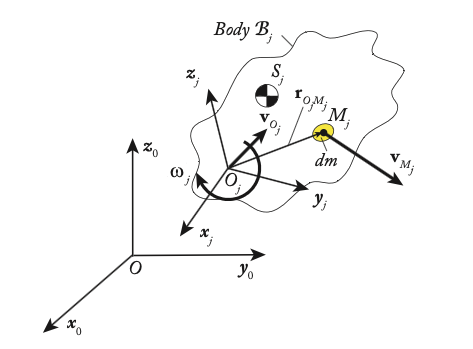
\includegraphics[scale=0.55]{images/rigid-body.png}\hfill
    \caption{Schematic of a rigid body}\hfill
    \label{fig: rigid-body}
\end{figure}

From equations \ref{eq: NE}, the sum of forces and sum of moments at CoM are given by,

\begin{align}
    \begin{split}
        \sum f_j &= \frac{d}{dt}|_{\mathcal{F}_j}p_j 
                = m_j\dot{v_{CoM_j}} \\
        \sum m_j &= \frac{d}{dt}|_{\mathcal{F}_j} (\mathbf{I}_{CoM_j} \omega_j) 
                =\mathbf{I}_{CoM_j}\dot{\omega_j} + \omega_j \times (I_{CoM_j}.\omega_j)
    \end{split}
\end{align}

where $\dot{v_{CoM_j}}$ is the acceleration of the CoM of body $j$; $\dot{\omega_j}$ is the angular acceleration of the body $j$ and 
$\mathbf{I_{CoM_j}}$ is the inertia matrix of body $j$. The NE equations can also be expressed at the origin $\mathcal{O}$ to the body 
$\mathcal{B}_j$ can be expressed as proposed in \cite{khalil2004modeling} as


\begin{align}
    \begin{split}
        \sum f_j &= m_j\dot{v_j} + \dot{\omega_j} \times ms_j + \omega_j \times (\omega_j \times ms_j)\\
        \sum m_j &= \mathbf{I}_{\mathcal{O}}\dot{\omega_j} + \omega_j \times (I_{\mathcal{O}}.\omega_j) + ms_j \times \dot{v_j}
    \end{split}
    \label{eq: NE-rigid-origin}
\end{align}

where $ms_j = m_j.r_{\mathcal{O}CoM_i}$ is the vector of first moment of inertia and $\mathbf{I}_{\mathcal{O}}$ is the inertia matrix at origin $\mathcal{O}$.
Using the screw notation, equation \ref{eq: NE-rigid-origin} can be rewritten as,


\begin{align}
    \sum w_j = \begin{bmatrix}
        \sum f_j \\
        \sum m_j
    \end{bmatrix} &= 
    \begin{bmatrix}
        m_j\mathcal{I}_3 & \hat{ms_j}^T \\
        \hat{ms_j}^T & I_{\mathbf{O}}
    \end{bmatrix}
    \begin{bmatrix}
        \dot{v_j} \\
        \dot{\omega_J}
    \end{bmatrix} +
    \begin{bmatrix}
        \omega_j \times (\omega_j \times (\omega_J \times ms_j)) \\
        \omega_j \times (I_{\mathcal{O}}\omega_j)
    \end{bmatrix} &= M_j\dot{q} + c_j
    \label{eq: ddm}
\end{align}

where $\mathcal{I}_3$ is the identity matrix of size $3$, $M_j$ is the generalized inertial matrix of body $\mathcal{B}_j$ and $c_j$ is the vector of Coriolis and centrifugal effects.
$\sum w_j$ (alias $\varGamma$) is the wrench representation which holds the sum of forces and moments and the equation \ref{eq: ddm} represent the direct dynamic model for a system.
Then the inverse dynamic model can be given by,

\begin{equation}
    \dot{q} = M_j^{-1}(\varGamma - c_j)
\end{equation}

\subsection{Multi body dynamics}

For modelling multi-body dynamics or tree-structured systems in this case, recursive NE algorithm is the most efficient problem than the recursive Lagrangian equations \cite{khalilunified}.

\begin{figure}[h!]
    \centering
    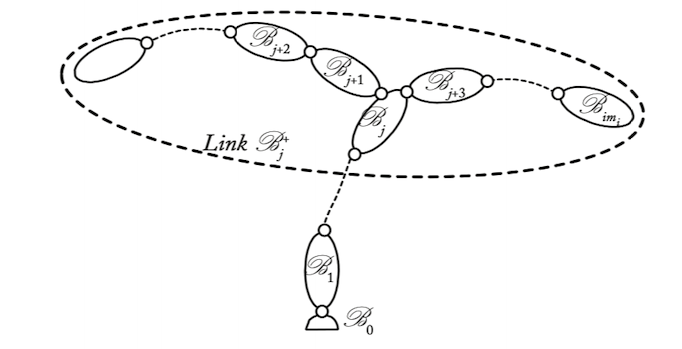
\includegraphics[scale=0.5]{images/multi-rigid-body.png}\hfill
    \caption{Rigid-body representation of tree structured model}\hfill
    \label{fig: tree-rigid-body}
\end{figure}

The recursive algorithm for multi-body system adapted from equation \ref{eq: NE-rigid-origin} is given by \cite{khalilunified}

\begin{align}
    \begin{split}
        \sum f_i &= f_i - \sum_r f_r + m_i\mathbf{g} - f_e \\
        \sum m_i &= m_i - \sum_r (R_km_k + r_k \times f_k) + ms_i \times \mathbf{g} - m_e 
    \end{split}
\end{align}

where $r_k = r_{\mathcal{O}k}$ is the distance vector from origin to force points on body $\mathcal{B}_i$; $ms_i \times \mathbf{g} = r_{\mathcal{O}CoM} \times m_i\mathbf{g}$
$f_r$ and $m_r$ are the reaction forces and moments respectively exerted by the body $\mathcal{B}_r$ on the body $\mathcal{B}_i$ at point $\mathcal{O}_r$;
$f_e$ and $m_e$ represent the forces and moments exerted on the environment by body $\mathcal{B}_i$. These values are assumed to be known.

\subsection{Dynamic Model of NAO robot}

This section derives the dynamic model of the humanoid robot NAO considering the absence of force sensors in the robot feet. 
The mass, CoM and Inertial matrices of the NAO robot v5 H25 is documented on the aldebaran website \cite{aldebaran-masses}. The mass and coordinates of CoM of individual 
links are taken and processed. The CoM given in the documentation is presented relatively to a local coordinate system $\mathcal{R}_j$ attached to the corresponding body $\mathcal{B}_j, i={1, 2, ..., 25}$.
To define the frame system corresponding to the modified DH rule, one has to rotate, translate or do both to compensate the new model for 
inverse dynamics model.

Let $CoM_j^A = [x_A, y_A, z_A]^T$ be the coordinates of the local reference frame $\mathcal{R}_j$ specified in the documentation \cite{aldebaran-masses}. Then the inertial tensor
considering the system of particles of the body about the center of mass with $r=xyz$ as the position vector is defined as,

\begin{equation}
    \label{eq: inertial-tensor}
    J_j^j = \begin{bmatrix}
        \int(y^2 + z^2)dm && -\int xydm && -\int xzdm \\
        -\int xydm && \int (x^2 + z^2)dm && -\int yz dm \\
        -\int xz dm && -\int yz dm && -\int(x^2 + y^2) dm
    \end{bmatrix} 
\end{equation}

\begin{figure}[h!]
    \centering
    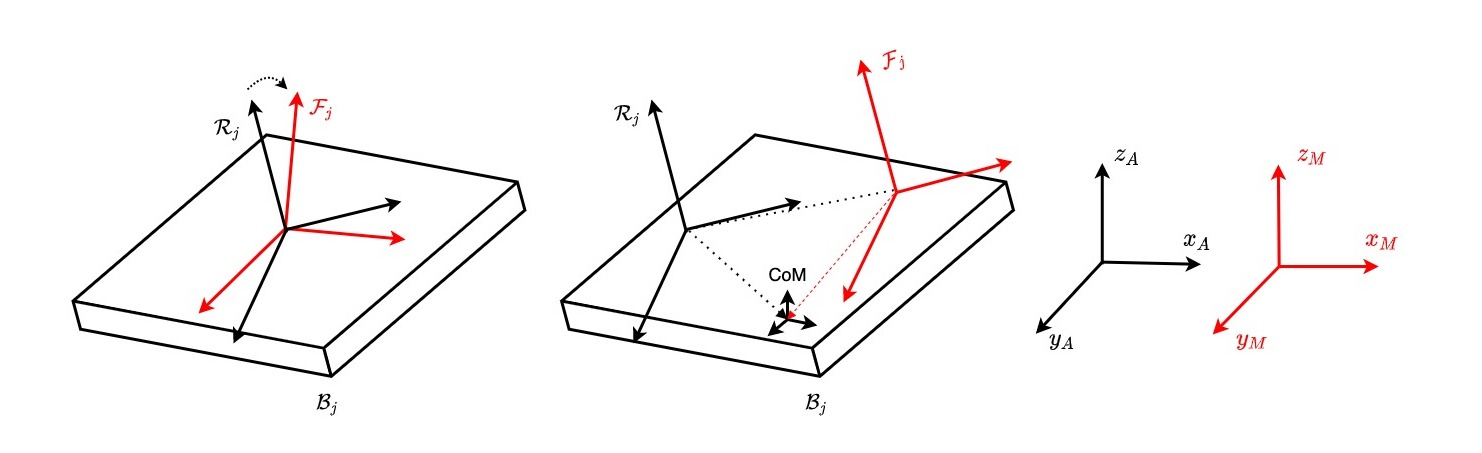
\includegraphics[scale=0.35]{images/flowchart-transformation-frames.jpg}\hfill
    \caption{Rotation and Translation of Body reference frame}\hfill
    \label{fig: body-frame-transformation}
\end{figure}

Since the matrix in equation \ref{eq: inertial-tensor} depends on the coordinates of the CoM, when the reference frame changes, the value of inertial tensors changes automatically \cite{karthikmunirathinam}.
To perform rotation from the provided CoM coordinate $CoM_j^A$ represented from $\mathcal{R}_j$ to the coordinate $CoM_j^M$ represented in $\mathcal{F}_j$, the rotation matrix is defined and the rotation matrix
can be computed as,

\begin{equation}
    \label{eq: rotation-frame}
    ^AJ = {^M}A_A{^A}J({^M}A_A)^T
\end{equation}

and the translation can be computed by \cite{karthikmunirathinam},

\begin{align}
    \label{eq: translation-frame}
        {^M}J + m \begin{bmatrix}
            y^2_A + z^2_A && -x_Ay_A && -x_Az_A \\
            -y_Ax_A && x^2_A + z^2_A && -y_Az_A \\
            -z_Ax_A && -z_Ay_A && x^2_A+y^2_A
        \end{bmatrix} = {^A}J + m \begin{bmatrix}
            y^2_M + z^2_M && -x_My_M && -x_Mz_M \\
            -y_Mx_M && x^2_M + z^2_M && -y_Mz_M \\
            -z_Mx_M && -z_My_M && x^2_M+y^2_M
        \end{bmatrix}
\end{align}


Once the frames are transformed to the respective notation, recursive Newton-Euler formalism of dynamic equation from section \ref{rigid-body-dynamics}
can be used to formulate the dynamic model of the equations.

% \subsection{Centroidal dynamics of humanoid robot}

\subsection{Zero Moment Point (ZMP)}

The zero moment point (ZMP) of the legged system can be defined as a point where the reaction force at the contact 
of the foot with the ground doesn't produce any horizontal moment i.e., the point where the total of horizontal inertia and
gravity forces equals zero. ZMP is useful in defining the stability criterion of the legged system using the support polygon of 
the foot. A support polygon is a region of perpendicular projection of the balancing end-effectors (legs) that carry the robot's weight.
A ZMP is a projection of the CoM onto the support polygon and it should lie within the region. Any attempt for the ZMP 
outside the support polygon to an extent will result in robot fall. Having these considerations, the ZMP of a biped system
can be given by,

\begin{equation}
    \begin{split}
        P_{ZMP} = P_{CoM} - \ddot{P}_{CoM}(\frac{z_{CoM} - z_{ZMP}}{\mathbf{g} + \ddot{z}_{CoM}})
    \end{split}
\end{equation}

where $\mathbf{g} = -9.81 m/s^2$ is the gravity acceleration. Fixing these points onto a specific position on the floor is 
over-constraining and leaves less free DOF for the other tasks. However, this precise control over the point positioning is advantageous
for choosing safer positions far from the foot’s edges and for avoiding points too far from the ankle which would require too much torque
to hold the whole body \cite{louisepouble}.


\section{Control Approach}

Proposing a control approach for a humanoid robot imitating the human actor differs from standard humanoid control approaches since 
feedback from both human and humanoid robot needs to be taken into account. This section explains the concepts and the approach 
carried out for humanoid control for motion imitation using Stack of Tasks (SoT).

\subsection{Balance Control}
\label{sec: balance-control}
\subsubsection{CoM Retargetting}

To track the Centre of Mass (CoM) of the human actor, an implementation from \cite{penco:hal-01895145} is adapted to track the normalized offset on
human's CoM relative to the support feet. For this case, a projection on 2D plane is considered. The human CoM $P_{CoM}, H$ can be 
expressed using modified Hanavan Model approximation. The normalized offset $\mathbf{o}$ between 0 and 1 can be computed as follows.


\begin{figure}[h!]
    \centering
    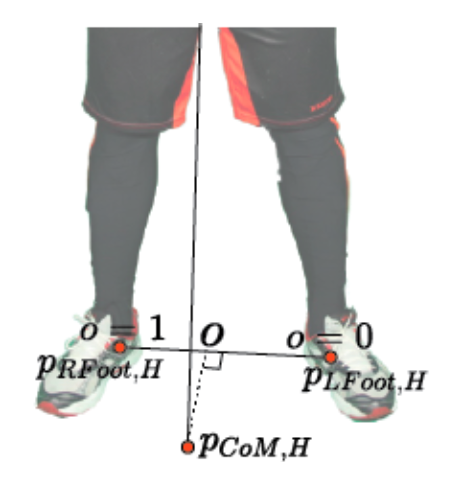
\includegraphics[scale=0.4]{images/human-com-track.png}\hfill
    \caption{Representation of offset projection of human actor \cite{penco:hal-01895145}}\hfill
    \label{fig: human-com-offset}
\end{figure}

\begin{equation}
    \mathbf{o} = \frac{(P_{CoM, H}) - P_{LFoot, H})(P_{RFoot, H} - P_{LFoot, H})}{||P_{RFoot, H} - P_{LFoot, H}||^2}
    \label{eq: human-com-offset}
\end{equation}

where $P_{CoM, H}$ represent the position of CoM projection of human actor. on the horizontal plane; $P_{LFoot, H}$ and $P_{RFoot, H}$ are the position of 
the left and right foot of the human actor respectively. The normalized offset $\mathbf{o}$ has an value of 0.5 during double support and has 0 or 1 
during single support. The robot CoM projection then is calculated as,

\begin{equation}
    P_{CoM, R} = P_{LFoot, R} + \mathbf{o}(P_{RFoot, R} - P_{LFoot, R})
    \label{eq: robot-com-1}
\end{equation}

To retarget also changes of the human CoM that are not on the line connecting the two feet, we first measure the maximum backward and forward CoM displacement
 of the human and of the robot over their support polygon (with the origin lying on the feet line), i.e $\delta_{CoM_{back}, H}, \delta_{CoM_{forw}, H}, \delta_{CoM_{back}, R}$ and 
$\delta_{CoM_{forw}, R}$ respectively. Then the retargetting the human CoM displacement $\vartriangle_{CoM, H}$ within the range such that $-\delta_{CoM_{back}, H} \leq 
 \vartriangle_{CoM, H} \leq \delta_{CoM_{forw}, H}$ can be computed as ,

 \begin{equation}
     \mathbf{o'} = \frac{(\vartriangle_{CoM, H} - (-\delta_{CoM_{back}, H}))}{(\delta_{CoM_{forw}, H} - (-\delta_{CoM_{back}, H}))}
 \end{equation}

 for which the robot CoM displacement is

 \begin{equation}
     \vartriangle_{CoM, R} = \mathbf{o'}(\delta_{CoM_{forw}, R} + \delta_{CoM_{back}, R}) - \delta_{CoM_{back}, R}
 \end{equation}

This displacement is then used in the orthogonal direction of the line connecting the two feet of the robot.

\subsubsection{Floating base Control}

To control the height of the floating base of the robot,, the pelvis point of the human actor is considered. The deviation of the pelvis point of the human is given by,

\begin{equation}
    \vartriangle_{base_{t, H}} = base_{t,H} - base_{0, H} 
\end{equation}

where $t$ is the timestep such that $t \geq 0$. Then the correction for robot base is given by,

\begin{equation}
    \vartriangle_{base_{t, H}} = \frac{h_{base, R}}{h_{base, H}} \vartriangle_{base_{t, R}}
\end{equation}


where $\alpha =  \frac{h_{base, R}}{h_{base, H}} $ is the ratio of height of the floating base of the robot and of the pelvis of the human,
at N-pose. Then the height of the robot base at each timestep can be calculated by,


\begin{equation}
    base_{t, R} = base_{0,R} + \vartriangle_{base_{t, R}}
\end{equation}


The change of orientation of the floating base is also calculated in a similar way, by computing the roll, pitch and yaw from the quaternion information given by the motion capture system.

\subsubsection{ZMP Retargetting}

During whole body teleoperation of humanoid robots, disastrous crashes may occur if the desired CoM trajectories recorded from the human do not ensure the balance of the controlled robot when retargeted.

To this scope, we propose a QP-based “preprocessor” that adjusts in real-time the desired commanded CoM to satisfy constraints that represent a condition for dynamic balance. In order to achieve a stable CoM trajectory we employ the linear inverted pendulum model (LIPM) in combination with the Zero Moment Point (ZMP) criterion.
The ZMP is represented with a point on the ground plane where the tipping moments, generated by the gravity and the inertial forces, are equal to zero. A humanoid robot keeps its balance if the ZMP is contained inside the support polygon of the robot.

Through the LIPM model it is possible to establish a simple relation between the ZMP and the CoM dynamics:

\begin{equation}
    \ddot{p}_{CoM} = \frac{g}{h}(p_{CoM} - p_{ZMP})
    \label{eq: zmp-control}
\end{equation}

\subsection{Posture Control}
\label{sec: posture-control}

This section provides a method for the simplification of humanoid robot and the human actor as a composition of inverted pendulum models. These simplified multi-double inverted pendulum models are used for posture control
during the motion retargetting.

\subsubsection{Multi-Double Inverted Pendulum Model (M-DIP)}
The full humanoid robot may be simplified using a combination of different double inverted pendulums as represented in figure \ref{fig: human-mdip}. The current position of the individual pendulums is represented as $\mathbb{P}_i$ and $\mathbf{P}_i$ for
human actor and humanoid respectively where i represent the left hand ($lh$), right hand ($rh$), right leg ($rl$) and left leg ($ll$). Then the state of the human actor $\mathbb{P}$ and humanoid robot $\mathbf{P}$ is represented as, 


\begin{align*}
    \label{eq: pendulum-state}
        \mathbb{P} = \begin{bmatrix} \mathbb{P}_{rh} && \mathbb{P}_{rl} && \mathbb{P}_{lh} && \mathbb{P}_{ll} \end{bmatrix}^T \qquad
        \mathbf{P} = \begin{bmatrix} \mathbf{P}_{rh} && \mathbf{P}_{rl} && \mathbf{P}_{lh} && \mathbf{P}_{ll} \end{bmatrix}^T
\end{align*}


\begin{figure}[h!]
    \centering
    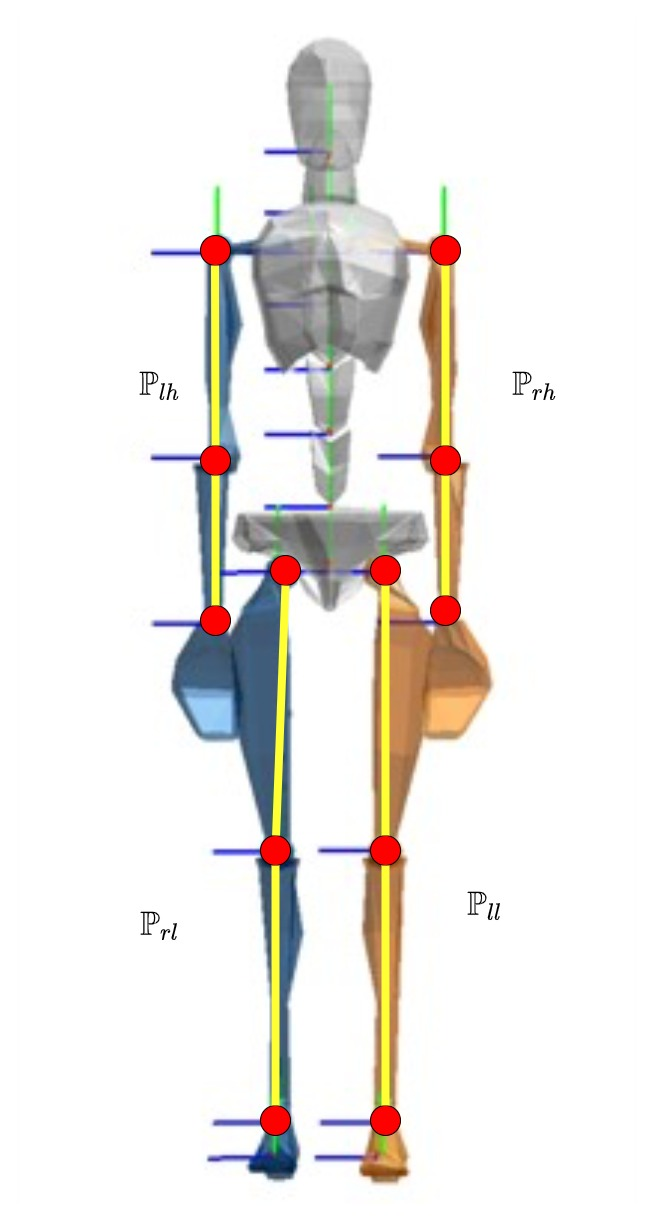
\includegraphics[scale=0.25]{images/flowchart-xsens-pendulum.jpg}\hfill
    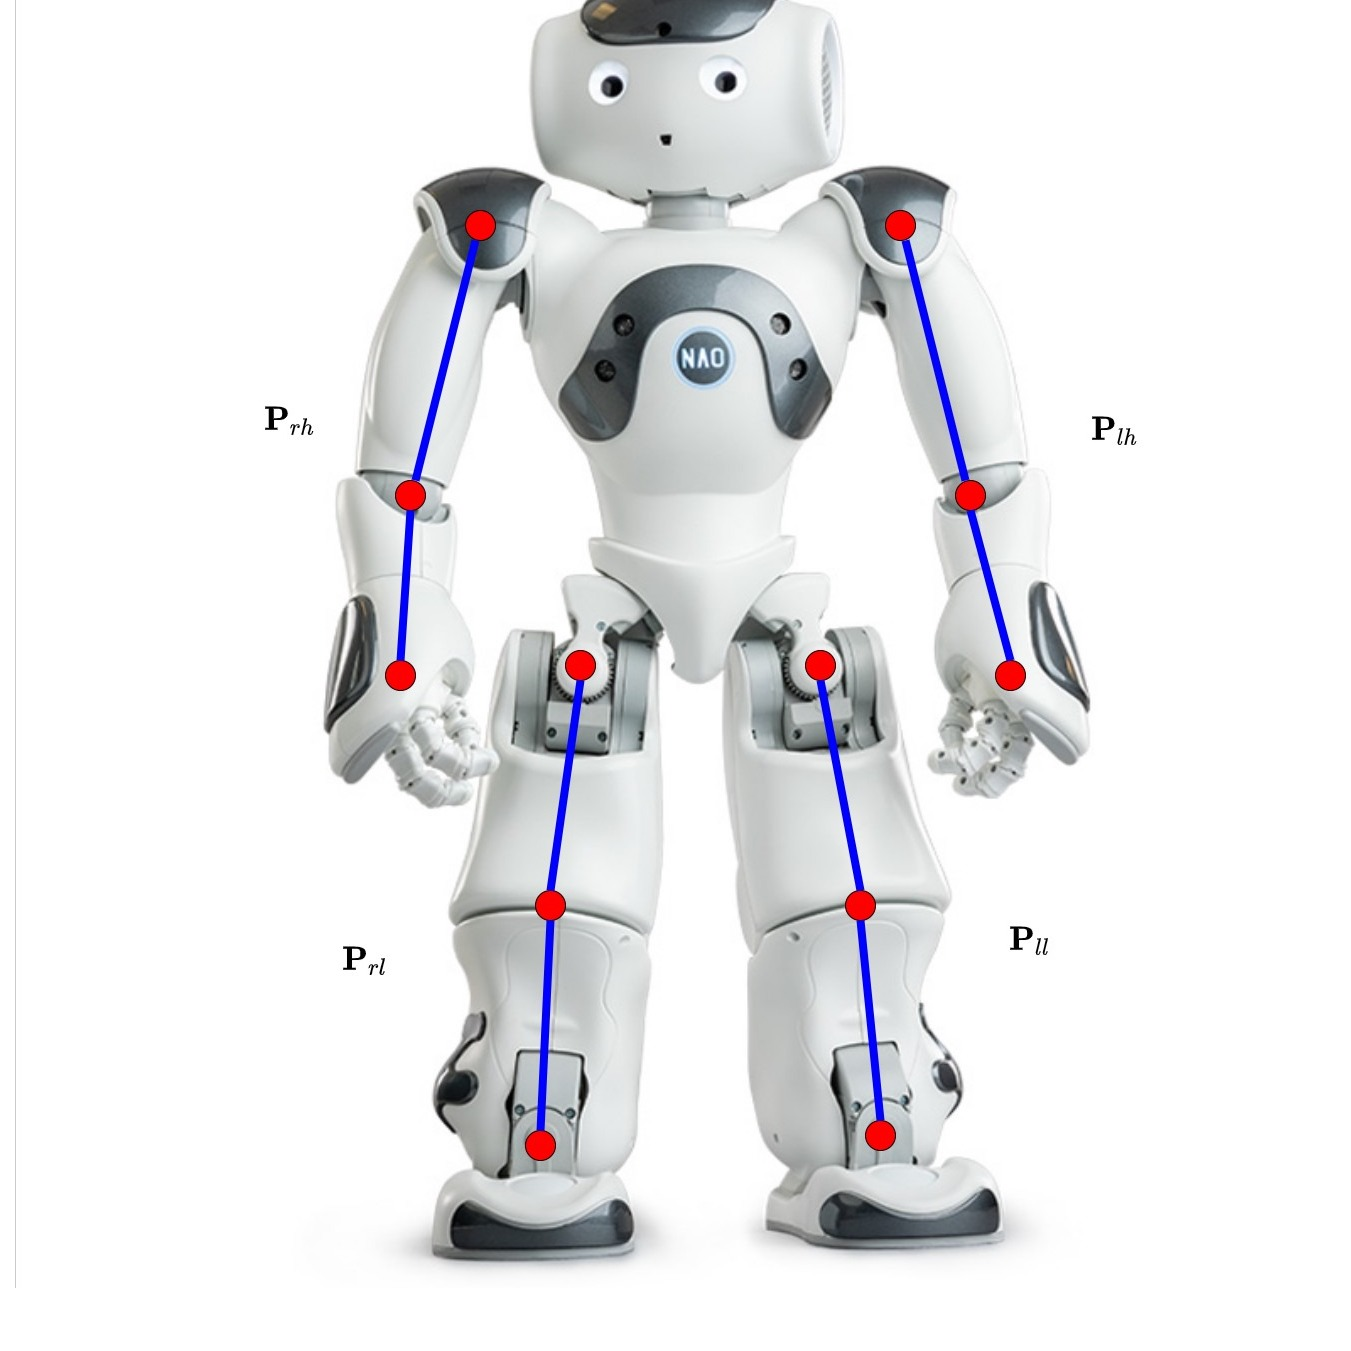
\includegraphics[scale=0.2]{images/flowchart-NAO-pendulum.jpg}\hfill
    \caption{Human actor and NAO robot as M-DIP model }\hfill
    \label{fig: human-mdip}
\end{figure}

The individual pendulums states are comprised of roll and pitch angles in the robot frame and can be used the formulate the equation of motions from equation \ref{eq: inverse-dynamic-model} \cite{pierro2012stabilizer}.
The mass, velocity and acceleration contribution of the M-DIP as composition can be computed as,

Mass:
\begin{equation}
    \label{eq: MDIP-mass}
    \mathbb{M} = m_{rl} + m_{ll} + m_{rh} + m_{rh}
\end{equation}

Velocity:
\begin{equation}
    \label{eq: MDIP-velocity}
    \mathbb{\dot{X}}_i = m_il_{sl}l_i\begin{bmatrix}
        0 && -\sin(\gamma_{sl} - \gamma_i)\dot{\gamma}_i \\
        \sin(\alpha_{sl} - \alpha_i)\dot{\alpha}_i && 0
    \end{bmatrix} \qquad \mathit{,i = rh, rl, lh, ll}
\end{equation}


Acceleration:
\begin{equation}
    \label{eq: MDIP-acceleration}
    \ddot{\mathbb{X}}_i = m_il_{sl}l_i\begin{bmatrix}
        0 && -\cos(\gamma_{sl} - \gamma_i) \\
        \cos(\alpha_{sl} - \alpha_i) && 0
    \end{bmatrix} \qquad \mathit{,i = rh, rl, lh, ll}
\end{equation}

where $i=sl$ represent the pendulum in contact with the environment (in this case, the legs); $\alpha_i$ and $\gamma_i$
represent the roll and pitch angles of the respective pendulums $i$ respectively. Given the velocity and acceleration contribution of the M-DIP to the composition model, the position of ZMP can also be retrieved
as, 

\begin{equation}
    \label{eq: MDIP-zmp}
    p_{ZMP, H} = \frac{1}{\mathbf{g}\mathbb{M}}\{\mathbb{\ddot{X}}\mathbb{\ddot{P}} + \mathbb{\dot{X}}\mathbb{\dot{P}} + \mathbb{M}l_{sl}\mathbf{g}\begin{bmatrix}
        \sin(\gamma_{sl}) \\
        -\sin(\gamma_{sl})
    \end{bmatrix}_{H}\}
\end{equation}

The equation \ref{eq: MDIP-zmp} can also be rewritten for calculating the postion of robot ZMP as,

\begin{equation}
    \label{eq: MDIP-robot-zmp}
    p_{ZMP, R} = \frac{1}{\mathbf{g}\mathbf{M}}\{\mathbf{\ddot{X}}\mathbf{\ddot{P}} + \mathbf{\dot{X}}\mathbf{\dot{P}} + \mathbf{M}l_{sl}\mathbf{g}\begin{bmatrix}
        \sin(\gamma_{sl}) \\
        -\sin(\gamma_{sl})
    \end{bmatrix}_{R}\}
\end{equation}

where,
\\
$\mathbb{P}_{i} = [-\arctan(\frac{-y_i}{z_i}) \quad \arctan(\frac{-y_i}{z_i})]^T$ is the position state of the respective pendulum $i$; \\
$\mathbb{\dot{X}} = [\mathbb{\dot{X}}_i, \mathit{i = rh, rl, lh, ll}]^T$ is the velocity contribution of the pendulum model of human; \\
$\mathbf{\dot{X}} = [\mathbf{\dot{X}}_i, \mathit{i = rh, rl, lh, ll}]^T$ is the velocity controibution of the pendulum model of robot; \\
$\mathbb{\ddot{X}} = [\mathbb{\ddot{X}}_i, \mathit{i = rh, rl, lh, ll}]^T$ is the acceleration contribution of the pendulum of human; \\
$\mathbf{\ddot{X}} = [\mathbf{\ddot{X}}_i, \mathit{i = rh, rl, lh, ll}]^T$ is the acceleration contribution of the pendulum of robot.

\subsubsection{Acceleration Control}

The human actor and the robot are simplified to the composition of M-DIP model and the posture control can be implemented directly using the acceleration feedback between the 
two subjects. The acceleration control for the motion-retargetting can be implemented as a weighted-constraint based problem \cite{van1985method},

\begin{equation}
    \label{eq: MDIP-control}
    \lim_{a \Rightarrow \infty} (HJ)^+ H\dot{e}^* = argmin (||H_iJ_i\dot{q} - H_i\dot{e}^*_i||^2), \quad \mathnormal{s.t. \quad J_i\dot{q} = \dot{e}_i^*}
\end{equation}


where 

